\documentclass[12pt]{article}
\usepackage{graphicx}
\usepackage[none]{hyphenat}
\usepackage{graphicx}
\usepackage{listings}
\usepackage[english]{babel}
\usepackage{graphicx}
\usepackage{caption} 
\usepackage{booktabs}
\usepackage{array}
\usepackage{amssymb} % for \because
\usepackage{amsmath}   % for having text in math mode
\usepackage{extarrows} % for Row operations arrows
\usepackage{listings}
\lstset{
  frame=single,
  breaklines=true
}
\usepackage{hyperref}
\usepackage{mathtools}

%Following 2 lines were added to remove the blank page at the beginning
\usepackage{atbegshi}% http://ctan.org/pkg/atbegshi
\AtBeginDocument{\AtBeginShipoutNext{\AtBeginShipoutDiscard}}


%New macro definitions
\newcommand{\mydet}[1]{\ensuremath{\begin{vmatrix}#1\end{vmatrix}}}
\providecommand{\brak}[1]{\ensuremath{\left(#1\right)}}
\providecommand{\sbrak}[1]{\ensuremath{{}\left[#1\right]}}
\providecommand{\norm}[1]{\left\lVert#1\right\rVert}
\providecommand{\abs}[1]{\left\vert#1\right\vert}
\newcommand{\solution}{\noindent \textbf{Solution: }}
\newcommand{\myvec}[1]{\ensuremath{\begin{pmatrix}#1\end{pmatrix}}}
\let\vec\mathbf


\begin{document}

\begin{center}
\title{\textbf{Convex Optimization}}
\date{\vspace{-5ex}} %Not to print date automatically
\maketitle
\end{center}
\setcounter{page}{1}

\section{12$^{th}$ Maths - Chapter 6}
This is Problem-1(i) from Exercise 6.5
\begin{enumerate}
\item Detrmine whether the function $f\brak{x} = \brak{2x-1}^2 + 3$ is convex or not. \\ 
\solution 
A single variable function $f$ is said to be convex if
\begin{align}
	\label{eq:convex_def}
	f\sbrak{\lambda x_1 + \brak{1-\lambda}x_2} \leq \lambda f\brak{x_1} + \brak{1-\lambda}f\brak{x_2},
\end{align}
for $\quad 0 < \lambda < 1$ and $x_1, x_2 \in \mathbb{R}$.

For a generic quadratic function $ax^2+bc+c$, let us determine the sufficient condition for it to be convex. Let 
\begin{align}
	\label{eq:Eq1}
	f\brak{x} &= ax^2+bx+c 
\end{align}
Substituting LHS of inequality from \eqref{eq:convex_def} in \eqref{eq:Eq1}
\begin{multline}
   \label{eq:Eq2}
	f\sbrak{\lambda x_1 + \brak{1-\lambda}x_2}  = f\sbrak{x_2 + \lambda \brak{x_1-x_2}}\\ 
	   =  a\sbrak{x_2+\lambda\brak{x_1-x_2}}^2 b\sbrak{x_2+\lambda\brak{x_1-x_2}} + c \\ 
	   = ax_2^2 + a\lambda^2 x_1^2+a\lambda^2 x_2^2 - 2a\lambda^2 x_1x_2 \\ 
	   +2a\lambda x_1x_2 - 2a\lambda x_2^2+bx_2+b\lambda x_1-b\lambda x_2+c 
\end{multline} 
Substituting RHS of inequality from \eqref{eq:convex_def} in \eqref{eq:Eq1}
\begin{multline}
	\lambda f\brak{x_1} + \brak{1-\lambda}f\brak{x_2}  = a \lambda x_1^2 + b\lambda x_1 + \lambda c \\ 
		 + \brak{1-\lambda}\brak{ax_2^2+bx_2+c} \\
	\label{eq:Eq3}
		= a \lambda x_1^2 + b\lambda x_1 + ax_2^2 + bx_2 + c -a\lambda x_2^2 -b\lambda x_2
\end{multline} 
Combining \eqref{eq:Eq2} and \eqref{eq:Eq3} with ineqiality and simplifying
\begin{align}
a\lambda^2 x_1^2 + a\lambda^2 x_2^2 - 2a\lambda^2 x_1x_2 +2a\lambda x_1x_2 - 2a\lambda x_2^2 \leq a\lambda x_1^2  -a\lambda x_2^2  
\end{align} 
\begin{multline}
	\label{eq:Eq4}
	a\lambda^2 x_1^2 + a\lambda^2 x_2^2 - 2a\lambda^2 x_1x_2 +2a\lambda x_1x_2 - a\lambda x_2^2 - a\lambda x_1^2 \leq 0 \\ 
	   x_1^2\brak{a\lambda^2-a\lambda} + x_2^2\brak{a\lambda^2 - a\lambda} - 2x_1x_2\brak{a\lambda^2-a\lambda} \leq 0 \\ 
	   \brak{a \lambda^2-a\lambda}\brak{x_1-x_2}^2 \leq 0\\
	   a\lambda\brak{1-\lambda}\brak{x_1-x_2}^2 \geq 0
\end{multline}
For the ineqality in \eqref{eq:Eq4} to be true,
\begin{align}
	a \geq 0 \because \lambda, 1-\lambda \geq 0, \brak{x_1-x_2}^2 \geq 0
\end{align}
However, $a \neq 0$, since it is a quadratice function. Hence $a > 0$, for $f\brak{x}$ to be convex.

The given function is 
\begin{align}
        \label{eq:Eq5}
	f\brak{x} &= \brak{2x-1}^2 + 3 \\ 
	&= 4x^2+4x+4 \\
	\therefore a &= 4, > 0
\end{align}
Hence, the function in equation \eqref{eq:Eq5} is convex.

The figure is as shown in Fig\ref{fig:Fig1}
\begin{figure}[!h]
	\begin{center}
		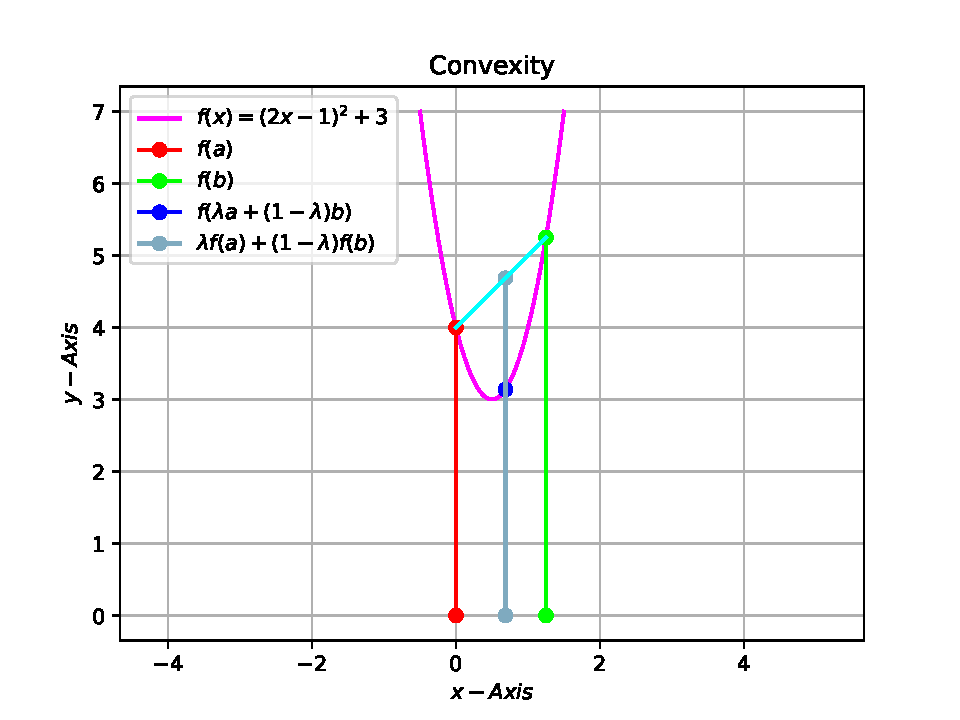
\includegraphics[width=\columnwidth]{figs/problem1.pdf}
	\end{center}
\caption{}
\label{fig:Fig1}
\end{figure}
\end{enumerate}
\end{document}
